\documentclass[a4paper]{scrreprt}

%% Language and font encodings and page settings
\usepackage[english]{babel}
\usepackage[utf8x]{inputenc}
\usepackage[T1]{fontenc}
\usepackage[a4paper,top=3cm,bottom=2cm,left=3cm,right=3cm,marginparwidth=2cm]{geometry}
\usepackage{float}

%% Packages
\usepackage{amsmath}
\usepackage{graphicx}
\usepackage[colorinlistoftodos]{todonotes}
\usepackage[colorlinks=true, allcolors=blue]{hyperref}

\title{Brexit Vs Good Friday}
\subtitle{"Defend the Good Friday Agreement"}
\author{Cian Gannon}
\titlehead{\centering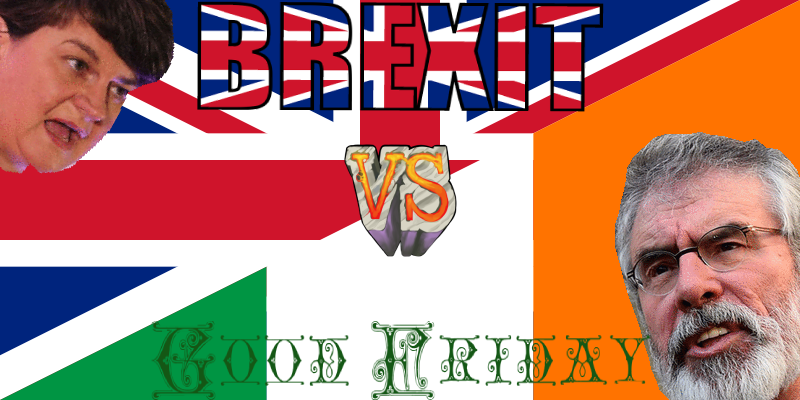
\includegraphics[width=10cm]{header}}

\pagestyle{headings}

\begin{document}

    \maketitle

    \begin{abstract}

        \centering
        
\includegraphics[width=2.7cm]{gerrylad}

        Brexit Vs Good Friday is a satirical representation of the current Brexit debacle and Ireland's core involvement in it due to the Good Friday Agreement. 
        Brexit Vs Good Friday is a top-down shooter that will expand the genre and also involve the most loved elements of other shooters.

        \begin{flushleft}
            \noindent
            \null\vfill
            Game Design Document \\
            Brexit Vs Good Friday \\
            \today \\
            Created by - Cian Gannon
        \end{flushleft}
        
    \end{abstract}

    \tableofcontents

    \chapter{Overview}

    \section{Main Concept}
    Brexit Vs Good Friday is a satirical representation of Brexit and the hysteria surrounding it. It's a top down shooter where the user plays Gerry Adams a politician who returns from retirement in order to save what many hold dear.
    
    \section{Core Selling Points}

        \subsection{Survival Elements}
            \begin{description}
                \item[$\bullet$] Player must dodge incoming fire.
                \item[$\bullet$] The aim of the game is to protect Good Friday in a countdown until the UK leaves the EU and the single market. If the player fails in their attempt by getting hit then Good Friday will be removed and the player fails. If the player survives the countdown then the Good Friday is upheld.
            \end{description}
        
        \subsection{Humor}
            \begin{description}
                \item[$\bullet$] The game is made to be humorous. It's take on Brexit that is a core issue currently in the EU is used to make all players on both sides laugh.
                \item[$\bullet$] The game is created to be topical, games that are topical tend to be a hit with players.
            \end{description}

        \subsection{Top Down Shooter}
            \begin{description}
                \item[$\bullet$] Top down shooter which needs basic input so the game will be comfortable to play on mobile or desktop.
                \item[$\bullet$] Top down games have been around for generations of consoles and have evolved over time. Brexit Vs Good Friday aims to take the general style and improve upon it.
            \end{description}

    \chapter{References} 

    \section{Games Examined}

        \subsection{GTA}

            \begin{figure}[H]
                \centering
                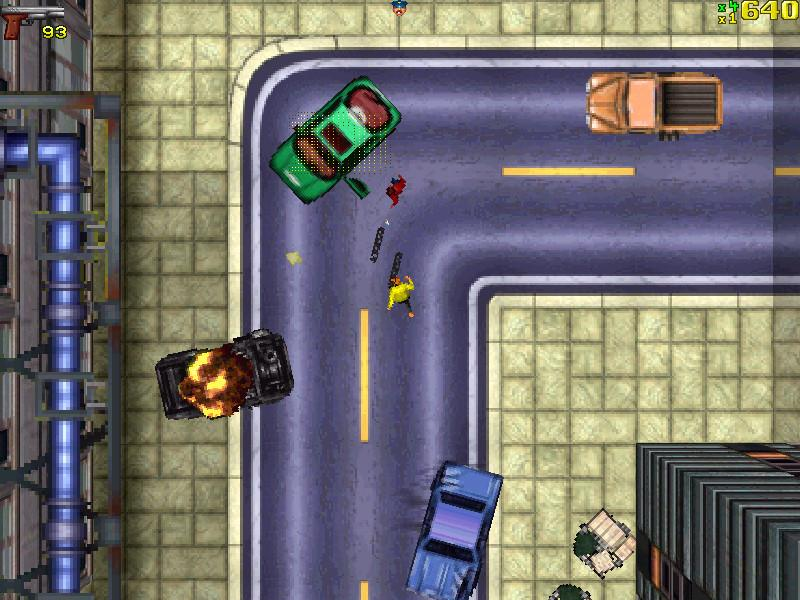
\includegraphics[width=0.70\textwidth]{gta1.jpg}
                \caption{\label{fig:art} GTA 1}
            \end{figure}

            \subsubsection{Core Features}
                \begin{description}
                    \item[$\bullet$] Single Player
                    \item[$\bullet$] Top Down Shooter
                    \item[$\bullet$] Open world
                    \item[$\bullet$] Action/Adventure
                    \item[$\bullet$] 2D
                \end{description}

                \subsubsection{Note}
                Grant Theft Auto is a top down action shooter developed by Rockstar Games. set in an open world approximation of Ney York city.
                A basic top down game that revolutionized the genre by adding an open world.
                What truely made Grand Theft Auto stand out from other game of the period are it's ease of use controls. 
                The pick up and play controls allowed users of all experience levels get to grips with game.
            
        \subsection{Doom}

            \begin{figure}[H]
                \centering
                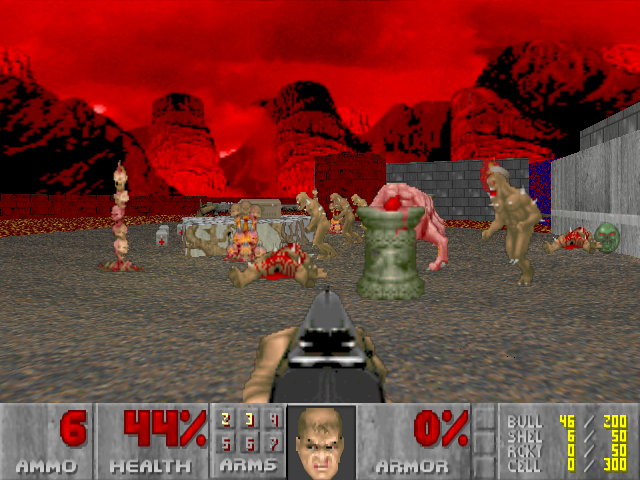
\includegraphics[width=0.70\textwidth]{doom.png}
                \caption{\label{fig:art} Doom}
            \end{figure}

            \subsubsection{Core Features}
            \begin{description}
                \item[$\bullet$] Single Player
                \item[$\bullet$] First Person Shooter
                \item[$\bullet$] Linear/Semi Open World
                \item[$\bullet$] Action
                \item[$\bullet$] 'Fake' 3D/ 2.5D
            \end{description}

            \subsubsection{Note}
            Doom is a first person shooter developed in 1993. 
            Although my game is going to be top down, taking inspiration from the first person shooter genre and adapting them for Brexit Vs Good Friday.
            Doom consists of constant stream of enemies in a fast paced enviroment that always keeps the player busy.
            Doom has no story and keeps the player entertained with gameplay alone.

        \subsection{Hotline Miami}

        \begin{figure}[H]
            \centering
            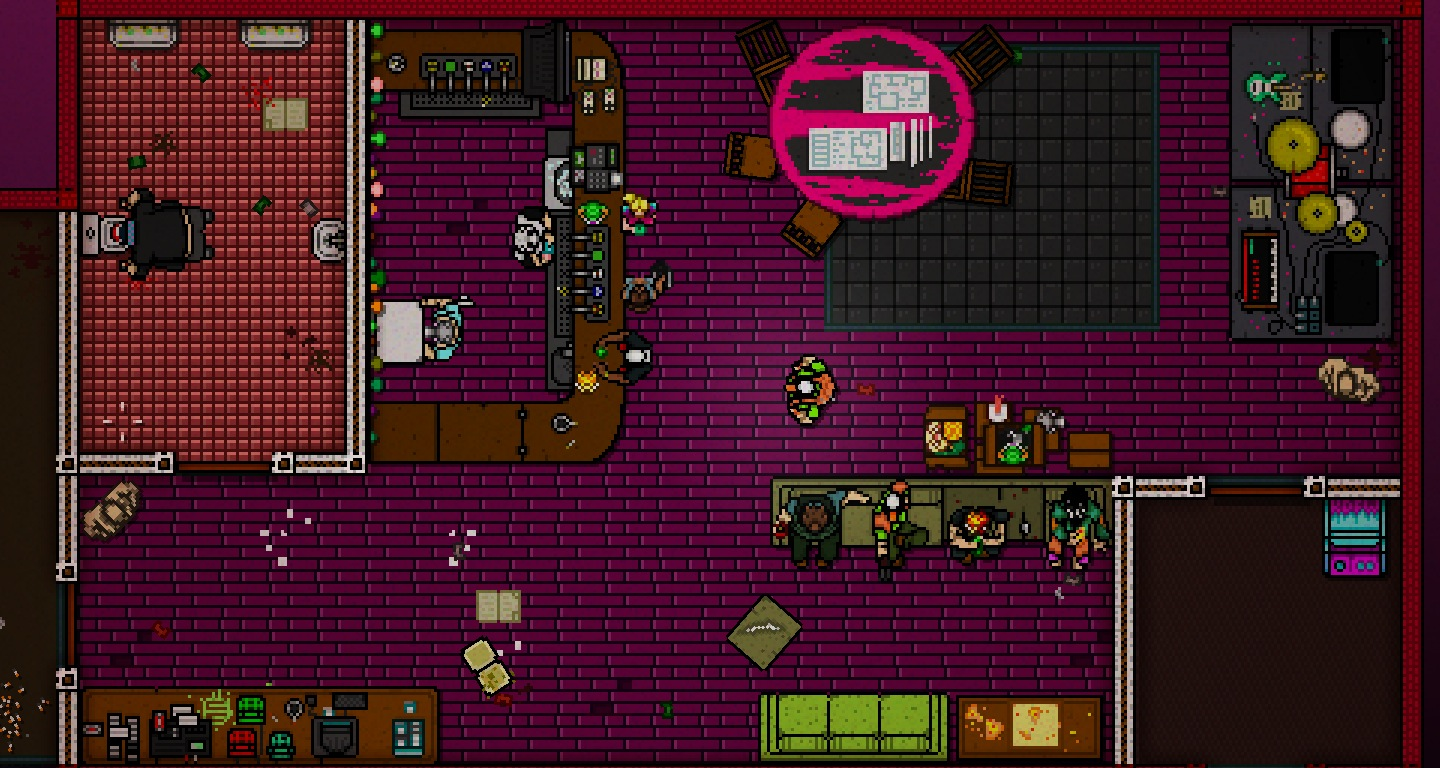
\includegraphics[width=0.70\textwidth]{hotline-miami.jpg}
            \caption{\label{fig:art} Hotline Miami}
        \end{figure}

        \subsubsection{Core Features}
        \begin{description}
            \item[$\bullet$] Single Player
            \item[$\bullet$] Top Down Shooter
            \item[$\bullet$] Semi Open World
            \item[$\bullet$] Action
            \item[$\bullet$] 2D
        \end{description}

        \subsubsection{Note}
        Hotline Miami is a top down action shooter that throws more and more enemies at the player in order to increase the difficulty for the player. 
        The player has a choice of wepaonry to deal with the onslaught of ever increasing enemies.   

    \chapter{Specification}

    \section{Target Group}

    \begin{description}
        \item[$\bullet$] The target group is a younger generation 35 and under who are interested in the currenct Brexit negotiations and just want to get away from the seriousness of it all.
        \item[$\bullet$] Target platform is mobile devices specifically windows phones.
    \end{description}

    \section{Genre}
    Brexit Vs Good Friday is a top down satirical shooter based on the current Brexit debate

    \section{Art Style}

    \begin{center}
        
\includegraphics[width=4.5cm]{celtic-knot}
        
\includegraphics[width=5cm]{celtic-knot-arrow}
        
\includegraphics[width=4.5cm]{celtic-knot}
        \begin{figure}[H]
            \centering
            
\includegraphics[width=4.5cm]{start-game}
            \caption{\label{fig:art} Game Menu Concept Art}
        \end{figure}
    \end{center}

    I'll be going for a traditional celtic art style as this game will portray the Irish viewpoint of Brexit. 
    It will mix celtic sybols for UI 'fluff' and use gaelic font type for menus.

    \begin{figure}[H]
        \begin{addmargin}[13.5em]{0em}
            
\includegraphics[width=1.5cm]{gerry-right}
            
\includegraphics[width=1.5cm]{arlene}
            
\includegraphics[width=1.5cm]{tess}
        \end{addmargin}
        \caption{\label{fig:art} Character Concept Art}
    \end{figure}

    \begin{flushleft}
        The game will use satirical representations of politicians throughtout the game as player characters and non player characters (NPCs).
    \end{flushleft}

    \begin{flushleft}
        The game will heavily lean on Irish humour surrounding our history and politics.
    \end{flushleft}

    \chapter{Gameplay and Setting}

    \begin{center}
        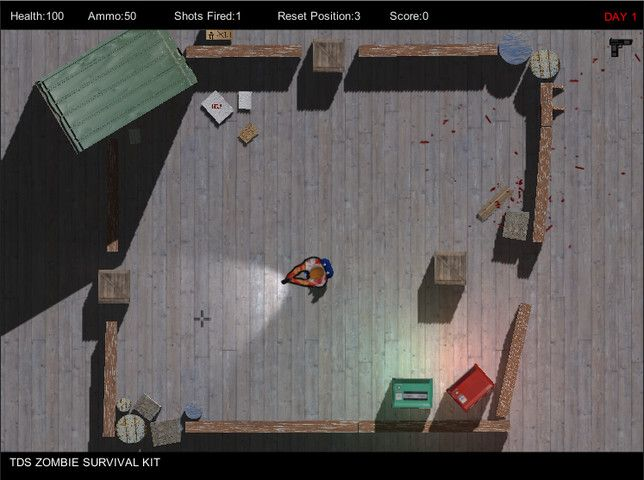
\includegraphics[width=7cm]{top-down}
    \end{center}

    The game is centered around the player who moved around the screen and defends against incoming enemies.
    The player will have special abilities that they may use in addition to their main offensive weapon.

    \section{Mood and Emotions}

    The mood of the game is to be humorous.
    The characters are over the top representations of real politicians the main menu will feature Irish in-jokes.
    The who premise of the game is to make the user laugh while also delivering compelling gameplay.

    \section{Objects in the Game}

    The players and the projectiles are the only objects in the game.

    \section{Characters in the Game}

    \begin{figure}[H]
        \begin{addmargin}[13.5em]{0em}
            
\includegraphics[width=1.5cm]{gerry-right}
            
\includegraphics[width=1.5cm]{arlene}
            
\includegraphics[width=1.5cm]{tess}
        \end{addmargin}
        \caption{\label{fig:art} Character Concept Art}
    \end{figure}

    The game will feature real world politicians in an over the top satirical outlook.
    The game will feature Gerry Adams as the main protaganist/antagonist (Depending on the users outlook)
    The game will use politicians from the UK as enemies that are trying to undermine the Good Friday Agreement.

    \section{Main Objective}

    Survive an onslaught of enemies while a counter is on screen.

    \section{Core Mechanics}

    \begin{description}
        \item[$\bullet$] Tactical Maneuvering \\
        Player will have to dodge incoming fire from enemies.
        \item[$\bullet$] Resource Management \\
        Player will have to manage their ammo and other abilities.
        \item[$\bullet$] Survival \\
        Player must survive hordes of enemies.
    \end{description}

    \section{Controls}

    \begin{center}
        
\includegraphics[width=7cm]{mobile}
    \end{center}

    The player will be controlled by using touchscreen on a mobile device.

\end{document}